\documentclass[10pt,a4paper]{report}
\usepackage[T1]{fontenc}
\usepackage{graphicx}
\usepackage{mathtools}
\usepackage{amsmath}
\usepackage[]{placeins}
\graphicspath{ {./img/} }

\begin{document}
	\section*{Ejercicio 1 - Convexidad}
	
	Recordamos del teórico que $f$ es convexa si $$f(t \cdot x + (1-t) \cdot y) \leq t \cdot f(x) + (1 - t) \cdot f(y) ,\hspace{6pt}   \forall x, y \in R^n, t \in [0,1]$$
	
	\subsection*{a) $g(x) = \sum_{i}^{} w_i f_i(x)$}
	
	$$g(x) = w_1 f_1(x) + w_2 f_2(x) + ... + w_k f_k(x)$$	
	
	$$g(t \cdot x + (1-t) \cdot y) = w_1 f_1(t \cdot x + (1-t) \cdot y) + w_2 f_2(t \cdot x + (1-t) \cdot y) + ... + w_k f_k(t \cdot x + (1-t) \cdot y)$$
	
	 Por convexidad de las funciones $f_i$ se cumple que
	$$g(t \cdot x + (1-t) \cdot y) \leq w_1 \left(t f_1(x) + (1-t) f_1(y)\right) + ... + w_k \left(t f_k(x) + (1-t) f_k(y)\right)$$
	
	Agrupamos los terminos multiplicados por $t$ por un lado y $(1-t)$ por otro
	$$g(t \cdot x + (1-t) \cdot y) \leq t \cdot \left[w_1 f_1(x) + w_2 f_2(x) + ... + w_k f_k(x)\right] + (1-t) \cdot \left[ ( w_1 f_1(y) + w_2 f_2(y) + ... + w_k f_k(y)\right]$$
	$$g(t \cdot x + (1-t) \cdot y) \leq t \sum_{i} w_i f_i(x) + (1-t) \sum_{i} w_i f_i(y) = t g(x) + (1-t) g(y)$$
	$\Rightarrow$ se cumple que g(x) es convexa.
	
	\subsection*{b) $l(x) = f_1(Ax + b)$}
	
	$$l(tx + (1-t)y) = f_1(A(tx + (1-t)y) + b)$$
	Observamos que $tb + (1-t)b = b$ por lo que lo incluimos en los respectivos terminos
	$$f_1(A(tx + (1-t)y) + b) = f_1(t (Ax + b) + (1-t) (Ay + b))$$
	
		Por convexidad de la función $f_1$ se cumple que
		$$l(tx + (1-t)y) =  f_1(t (Ax + b) + (1-t) (Ay + b))) \leq t f_1(Ax + b) + (1-t) f_1(Ay + b) = t l(x) + (1-t) l(y)$$
		$\Rightarrow$ l(x) es convexa.
		
	\subsection*{c) $Y = \cap_{i \in N} X_i$}
	
	Del teórico sabemos que un conjunto $C \subset R^n$ es convexo si se cumple:
	
	$$\forall x,y \in C,\hspace{6pt} tx + (1-t)y \in C, \forall t \in [0,1]$$
	
	Si tomamos dos puntos cualesquiera $(x,y)$ que pertenezcan a $Y$ sabemos por definición que también pertenecerán a la intersección de todos los $X_i$. Luego por convexidad de los $X_i$ esos puntos cumplen que $xt + (1-t)y \in X_i, \hspace{6pt} \forall i$ y, por ser $Y$ la intersección, $xt + (1-t)y \in Y$. Lo mismo aplica al tomar cualquier otro par $(x,y)\in Y$ $\Rightarrow$ $Y$ es convexa. 
	
	\subsection*{d) $ B(C,r) = \{x \in R^n : ||x-c|| \leq r\} $}
	
	Sean $x,y \in B(C,r)$ entonces debemos verificar si se cumple que $tx + (1-t)y \in B(C,r)$ o lo que es lo mismo, que 
	$||C - [tx + (1-t)y]|| < r$. 
	
	Partiendo de $[tx + (1-t)y]$, sabemos que
	
	$$||C - [tx + (1-t)y]|| = ||tC + (1-t)C - [tx + (1-t)y]|| = || t(C - x) + (1-t) (C - y) $$
	
	Utilizando la desigualdad triangular, se tiene que 
	
	$$||C - [tx + (1-t)y]|| \leq ||t(C-x)|| + ||(1-t)(C-y)|| = t\cdot||(C-x)|| + (1-t)\cdot||(C-y)||$$
	
	Ahora, sabemos que tanto $x$ como $y$ pertenecen a $B(C,r)$, con lo cual $||(C-x)|| < r$ y $||(C-y)|| < r$.
	
	Lo anterior se transforma entonces en
	
	$$||C - [tx + (1-t)y]|| \leq tr + (1-t)r = r$$
	
	Finalmente, verificamos que $[tx + (1-t)y] \in B(C,r)$ para cualquier par $x,y$ en $B(C,r)$ y $\forall t \in [0,1]$ 
	
	$\Rightarrow$ $B(C,r)$ es convexa.
	
	\section*{Ejercicio 2 - Interpretación geométrica}
	
	\subsection*{a) }
	
	Debemos probar que la función de costo $c(x,y) = -log(y^2 - x^2)$ es convexa. \\
	
	En primer lugar, se puede observar que $y^2 - x^2 = (y-x)(y+x)$. Por lo que $c(x,y) = -log(y^2 - x^2) = -log((y-x)(y+x))$.
	
	Luego, utilizando la sugerencia se obtiene:
	
	$$c(x,y) = -log(y-x)-log(y+x)$$
	
	Ahora podemos analizar cada termino de la suma por separado, analizar si es o no convexa. Pues, por resultado del ejercicio 1.a, suma de funciones convexas, es convexa. 
	
	Llamaremos $c_1(x,y) = -log(y-x)$ y $c_2(x,y) = -log(y+x)$, debemos analizar si la Hessiana es semidefinida positiva. 
	
	$$\frac{\partial^2 c_1}{\partial x^2} = \frac{1}{(y-x)^2}$$
	$$\frac{\partial^2 c_1}{\partial y^2} = \frac{1}{(y-x)^2}$$
	$$\frac{\partial^2 c_1}{\partial xy} = \frac{-1}{(y-x)^2}$$
	
	Observamos que $\frac{\partial^2 c_1}{\partial xy} = \frac{\partial^2 c_1}{\partial yx}$
	
	Su matriz Hessiana queda definida de la siguiente manera
	
	\[ H_{c_1} = \begin{bmatrix}
		\frac{1}{(y-x)^2} & \frac{-1}{(y-x)^2}\\
		\frac{-1}{(y-x)^2} & \frac{1}{(y-x)^2}
	\end{bmatrix} \]
	
	Y continuamos calculando sus valores propios:
	
	$$|H_{c_1} - \lambda I| = (\frac{1}{(y-x)^2}-\lambda)^2 - \frac{1}{(y-x)^4} = (\frac{1}{(y-x)^4}-\frac{2\lambda }{(y-x)^2} + \lambda^2 ) - \frac{1}{(y-x)^4}$$
	
	De lo anterior se deduce que $\lambda_1 = 0$ y $\lambda_2 = \frac{2}{(y-x)}$. Observamos que en el dominio de la función ($y > |x|$) ambos valores propios son no-negativos. Por lo tanto concluimos que $c_1(x,y)$ es convexa.
	
	Ahora observemos qué sucede con $c_2(x,y)$. En este caso tenemos
	
	$$\frac{\partial^2 c_1}{\partial x^2} = \frac{1}{(y+x)^2}$$
	$$\frac{\partial^2 c_1}{\partial y^2} = \frac{1}{(y+x)^2}$$
	$$\frac{\partial^2 c_1}{\partial xy} = \frac{1}{(y+x)^2}$$
	
	Observamos que $\frac{\partial^2 c_2}{\partial xy} = \frac{\partial^2 c_2}{\partial yx}$
	
	En el caso de $c_2$ se obtiene la siguiente matriz Hessiana
	
	\[ H_{c_1} = \begin{bmatrix}
		\frac{1}{(y+x)^2} & \frac{1}{(y+x)^2}\\
		\frac{1}{(y+x)^2} & \frac{1}{(y+x)^2}
	\end{bmatrix} \]
	
	Y sus valores propios se calculan a continuación
	
	$$|H_{c_1} - \lambda I| = (\frac{1}{(y+x)^2}-\lambda)^2 - \frac{1}{(y+x)^4} = (\frac{1}{(y+x)^4}-\frac{2\lambda }{(y+x)^2} + \lambda^2 ) - \frac{1}{(y+x)^4}$$
	
	De lo que se deduce que $\lambda_2 = 0$ y $\lambda_2 = \frac{2}{(y+x)^2}$. Por lo cual ambos valores propios son no-negativos y con ello, la matriz Hessiana es semidefinida positiva y se concluye que $c_2(x,y)$ es convexa.
	
	A partir de los resultados anteriores, demostramos que $c_1(x,y)$ y $c_2(x,y)$ son convexas, y por el resultado del ejercicio 1.a se concluye que $c(x,y)$ es convexa.
	
	\subsection*{b) }
	
	En primer lugar, podemos observar que la restricción $x^2 + y^2 \leq 1$ es lo mismo que decir que $(x,y) \in B(0, 1)$. Por el ejercicio 1d. podemos concluir que ese conjunto es convexo. Por otro lado, los conjuntos tales que $x \geq 0$, $2x-y \leq 0$, $y\geq 1/2$ son todos semiplanos. Los puntos pertenecientes a un hiperplano en $R^2$ son un conjunto convexo.
	
	\FloatBarrier 
	
	\subsection*{c) }
	
	\begin{figure}[!ht]
		\centering
		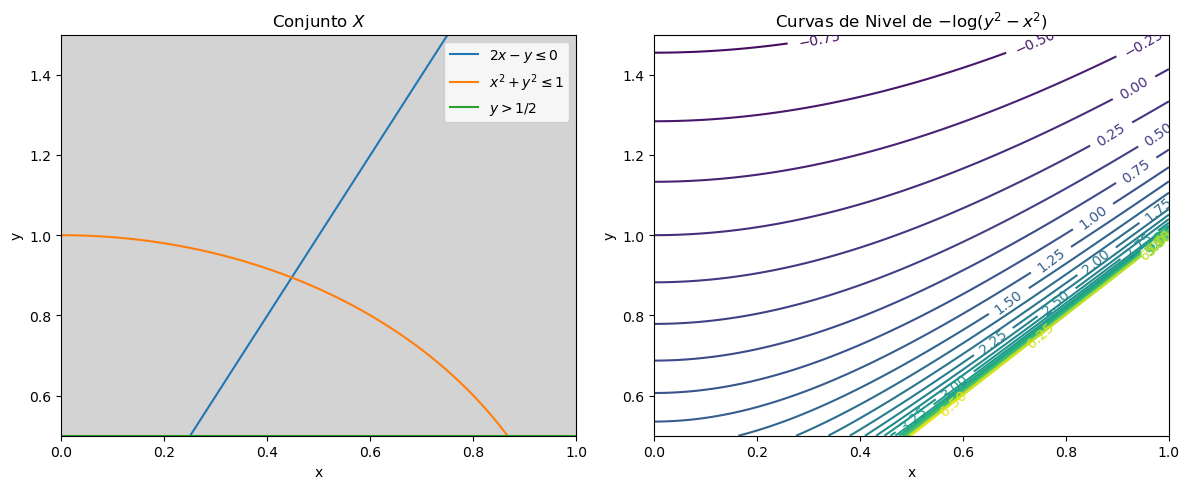
\includegraphics[width=1.2\textwidth]{ej2-1.png}
		\caption{Limites de la región factible a la izquierda. Curvas de nivel a la derecha.}
		\label{ej2-1}
		
	\end{figure}
	
	\begin{figure}[!ht]
		\centering
		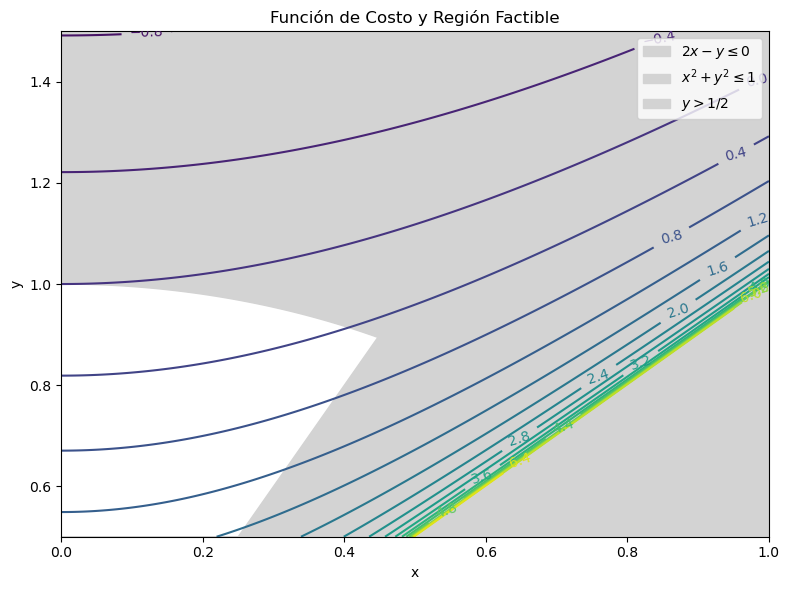
\includegraphics[width=1\textwidth]{ej2-2.png}
		\caption{Curvas de nivel, van de violeta a amarillo mientras más alto es su valor. Y en blanco se puede observar la región factible.}
		\label{ej2-2}
	\end{figure}
	
	\FloatBarrier 
	
	\subsection*{d) }
	
	Podemos observar los valores de las curvas de nivel, en particular, nos interesa la intersección de la curva de nivel correspondiente al valor cero con el conjunto factible. Si se observa de la Fig. \ref{ej2-2} la intersección de la curva de nivel correspondiente al valor funcional cero y la región factible (en blanco) se da en el punto $(x,y) = (0,1)$. Lo cual implica que ese punto es solución del problema.
	

\section*{Ejercicio 3 - Puntos críticos y óptimos globales}


	
	
\end{document}
